\chapter{Control}

Now that a functioning simulation environment is created a control hierarchy is needed. The initial thought is a multivariable control on top on single joint control. The multivariable control is done in Python or Matlab. The multivariable control will use the joint positions and joint velocities to compute the desired joint torques which is sent to joint PID controllers which is handled by using ROS control package. The first thing to do is therefore to create the individual joint PID controllers. 
To create these controllers two new files are needed. A new launch file must be created. It is possible to just append the launch file, but to make everything more understandable and if the package is to be used on the real robot it is easier to make a new launch file that can be included in other launch files. The task of the control.launch file is to spawn a node which includes all of the five controllers. In \lstref{lst:launchControl} one can see the the code to spawn the controllers. It consists of two statements. The first is loading the parameters of the controllers from the YAML file. Then with the parameters loaded, a node is created and it makes the joint controller services that the wanted joint torques can be published to. 
\begin{lstlisting}[language=xml,caption={Spawns the controller node},label={lst:launchControl}]
<rosparam file="$(find five_dof_robotarm)/config/joints.yaml" command="load"/>

  <node name="controller_spawner" pkg="controller_manager" type="spawner" respawn="false"
	output="screen" ns="/five_dof_robotarm" args="joint_state_controller
    base_to_turntable_controller
    second_joint_controller
    third_joint_controller
    fourth_joint_controller
    fifth_joint_controller"/>
\end{lstlisting}
Below in \lstref{lst:pythonPubl} one can see how the publishers that will publish the desired joint torques calculated by the controller. 
\begin{lstlisting}[language=python,caption={Python code for creating the publishers.},label={lst:pythonPubl}]
#Define publishers for each joint position controller commands.
pub1 = rospy.Publisher('/five_dof_robotarm/first_joint_controller/command', Float64, queue_size=10)
pub2 = rospy.Publisher('/five_dof_robotarm/second_joint_controller/command', Float64, queue_size=10)
pub3 = rospy.Publisher('/five_dof_robotarm/third_joint_controller/command', Float64, queue_size=10)
pub4 = rospy.Publisher('/five_dof_robotarm/fourth_joint_controller/command', Float64, queue_size=10)
pub5 = rospy.Publisher('/five_dof_robotarm/fifth_joint_controller/command', Float64, queue_size=10)
\end{lstlisting}

And how to publish the wanted torques is seen below in \lstref{lst:pythonPubs}. Here $u$ is the vector of the controller output. During the project it was also wanted to do the same in Matlab and the initial thought is the same and can be viewed in the appendix. 

\begin{lstlisting}[language=python,caption={Python code for publish wanted torques},label={lst:pythonPubs}]
pub1.publish(u[0,0])
pub2.publish(u[1,0])
pub3.publish(u[2,0])
pub4.publish(u[3,0])
pub5.publish(u[4,0])
\end{lstlisting}

Another important functionallity to do control is to get the feedback from Gazebo with joint position and joint velocities. To do this a subscriber is needed. The subscriber can thought of as the opposite as the publisher. Instead of publishing values to a service, we now want to listen to a service. 


\section{Control}

\subsection{PD controller with gravity compensation}

The controller that is going to be used is a simple PD controller with gravity compensation derived by \cite{spong}:
$$
    u=K_p\tilde{q} - K_d\dot{q} +g(q)
$$
 where $\tilde{q} = q_d - q$ and 
 \begin{align}\label{eq:gravity}
 g(q) = \frac{\partial P}{\partial q_k}
 \end{align}
 where the total potential energy for a n-link robot is $P = \sum^n_{i=1}P_i$. Where $P_i$ is the potential energy for each individual link. For this specific manipulator the center of mass is assumed in the geometric center of each link. In \cite{Siciliano} this controller is proven by using Lyapunov direct method to be globally asymptotically stable(GAS) as long as $K_d$ and $K_p$ is positive definite. It is important to keep in mind that if the online computing of $g(q)$ is not perfect, the statement of GAS does not hold. Based on the assumptions made, the controller can not guarantee GAS. 
 
 \subsection{Deriving the gravitational effect}
 The robot at hand starts and ends with twisting joints and only the three joints in the middle is rotational joints. This means that the potential energy is only dependent on $q_2$,$q_3$ and $q_4$ which makes calculating the potential energy a bit a easier. Because of this, the potential energy can be calculated by using a 2D sketch as shown in \figref{draw:pot-rob}.

\begin{figure}[htbp]
    \centering
    \input{tex/drawing/robotarm.tex}
    \caption{Sketch of the robot the three middle joints of the robot}
    \label{draw:pot-rob}
\end{figure}
     
In \eqref{eq:potE} the potential energy is calculated for each link in the robot. 
 \begin{align}
    \begin{split}\label{eq:potE}
        P_1 &= m_1g\frac{L_1}{2}
        \\
        P_2 &= m_2g\left(L_1 + \frac{L_2}{2}\cos{(q_2)}\right)
        \\
        P_3 &= m_3g\left(L_1 +  L_2 \cos{(q_2)} + \frac{L_3}{2}\cos{(q_2 + q_3)} \right)
        \\
        P_4 &= m_4g\left(L_1 +  L_2 \cos{(q_2)} + L_3\cos{(q_2 + q_3)} + \frac{L_4}{2}\cos{(q_2+q_3+q_4)} \right)
        \\
        P_5 &=m_5g\left(L_1 +  L_2 \cos{(q_2)} + L_3\cos{(q_2 + q_3)} + \left(L_4 + \frac{L_5}{2} \right)\cos{(q_2+q_3+q_4)} \right)
        \\
        P &= P_1 + P_2 + P_3 + P_4 + P_5
    \end{split}   
 \end{align}    


 Where $L_4$ is the part up to the rotational joint. $L_5$ and $m_5$ is the rotational joint and the gripper together.  \\
 
 And then, to calculate individual gravity components equation \eqref{eq:gravity} is used on \eqref{eq:potE}:

 \begin{align*}
    g_1 &= 0
    \\
    g_2 &= \frac{\partial P}{\partial q_2} = 
    m_2g\frac{L_2}{2}\sin{(q_2)}+
    m_3g\left( L_2 \sin{(q_2)} + \frac{L_3}{2}\sin{(q_2+q_3)} \right)\\&+
    m_4g\left( L_2 \sin{(q_2)} + L_3\sin{(q_2 + q_3)} + \frac{L_4}{2}\sin{(q_2+q_3+q_4)} \right)\\&+
    m_5g\left( L_2 \sin{(q_2)} + L_3\sin{(q_2 + q_3)} + \left(L_4 + \frac{L_5}{2} \right)\sin{(q_2+q_3+q_4)} \right)
    \\
    g_3 &= \frac{\partial P}{\partial q_3} =
    m_3g\frac{L_3}{2}\sin{(q_2+q_3)} +
    m_4g\left( L_3\sin{(q_2 + q_3)} + \frac{L_4}{2}\sin{(q_2+q_3+q_4)} \right)\\&+
    m_5g\left(  L_3\sin{(q_2 + q_3)} + \left(L_4 + \frac{L_5}{2} \right)\sin{(q_2+q_3+q_4)} \right)
    \\
    g_4 &=\frac{\partial P}{\partial q_4} = 
    m_4g\frac{L_4}{2}\sin{(q_2+q_3+q_4)}+
    m_5g\left(L_4 + \frac{L_5}{2} \right)\sin{(q_2+q_3+q_4)}
    \\
    g_5 &= \frac{\partial P}{\partial q_5} = 0
    \\
    g(q) &= [g_1,g_2,g_3,g_4,g_5]^T
 \end{align*}
This is the gravity components that each joint will \textit{feel} from the other links and by adding this to a PD controller it will compensate for this disturbance. 

\subsubsection{Test of controller}
Now that a controller is in place it is time to test it. The first thing to test is the gravity compensation. The best way to view the results is to watch the robot it is in a stationary state the only input that are sent into the individual joint torque controllers should be the data computed only by the gravity compensation part. Some random desired joint angles is chosen and the following results can be viewed in \tabref{table:gravity}.\\

\begin{table}[htbp]
\centering
\caption{Test results of the precision of the gravity compensation}
\label{table:gravity}
    \begin{tabular}{l c c r}
        \toprule
        Joint  &  $g_i$ & $u_i$ & $u_i-g_i$\\
        \midrule
        1 & 0 & 0 & 0\\
        2 & -0.7720  & -0.7760  & -0.0040 \\
        3 &-0.4226 & -0.4191 & 0.0035 \\
        4 & -0.1870 &-0.1871 & -0.0001\\
        5 & 0 & 0 & 0\\
        \bottomrule
    \end{tabular}
\end{table}

 One can see that the results are good. One can see that the PD part of the controller must some work which means that the end effector will not be completely at its desired position. The biggest error is in the second joint and for this configuration $0.0022 rad = 0.1261 deg$ which corresponds to an error of $0.0003$ in the xyz world frame. \\
 
Now that we know that the gravity compensation is working we can start to test the controller. The gain matrices $K_p$ and $K_d$ are implemented as positive definite diagonal matrices.

\begin{figure*}[htbp]
    \centering
    \begin{subfigure}[htbp]{0.45\textwidth}
        \centering
        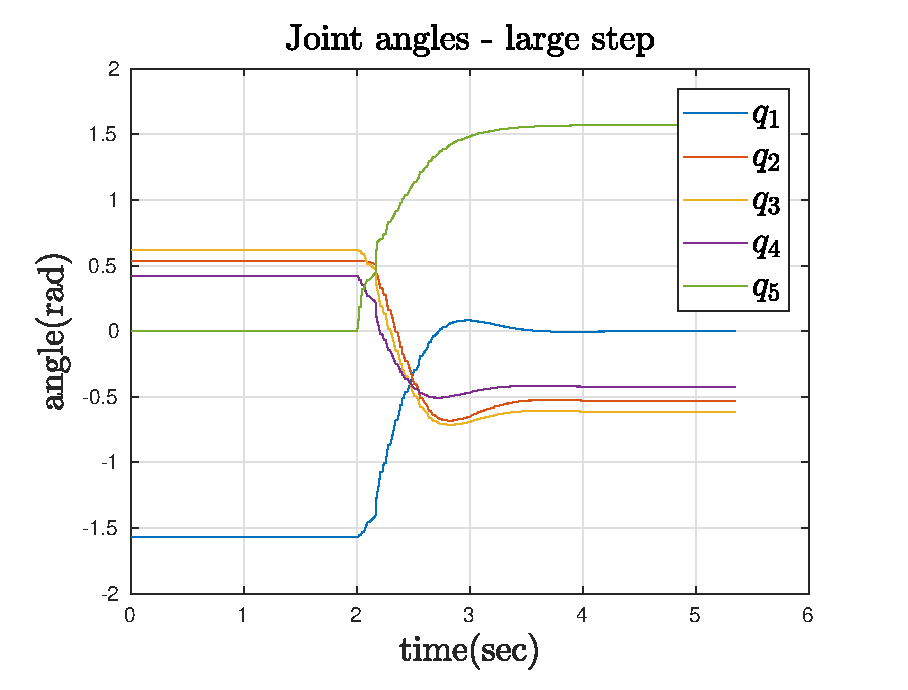
\includegraphics[width = 1.15\linewidth]{img/LSq.eps}
        \caption{ }
        \label{fig:LSq}
    \end{subfigure}
    ~ 
    \begin{subfigure}[htbp]{0.45\textwidth}
        \centering
        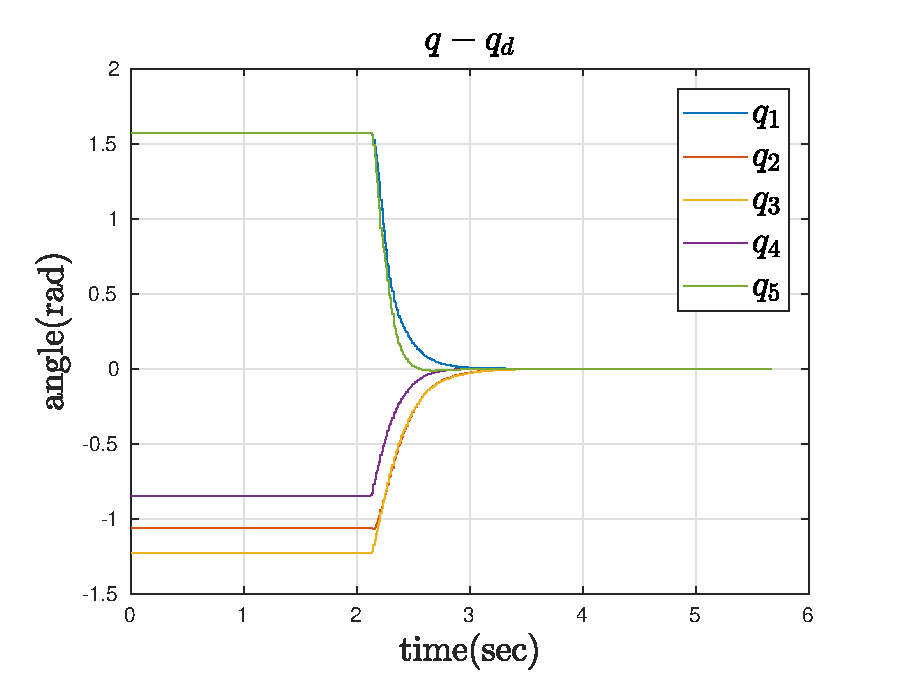
\includegraphics[width = 1.15\linewidth]{img/LSerror.eps}
        \caption{ }
    \end{subfigure}
    ~
    \centering
    \begin{subfigure}[htbp]{0.45\textwidth}
        \centering
        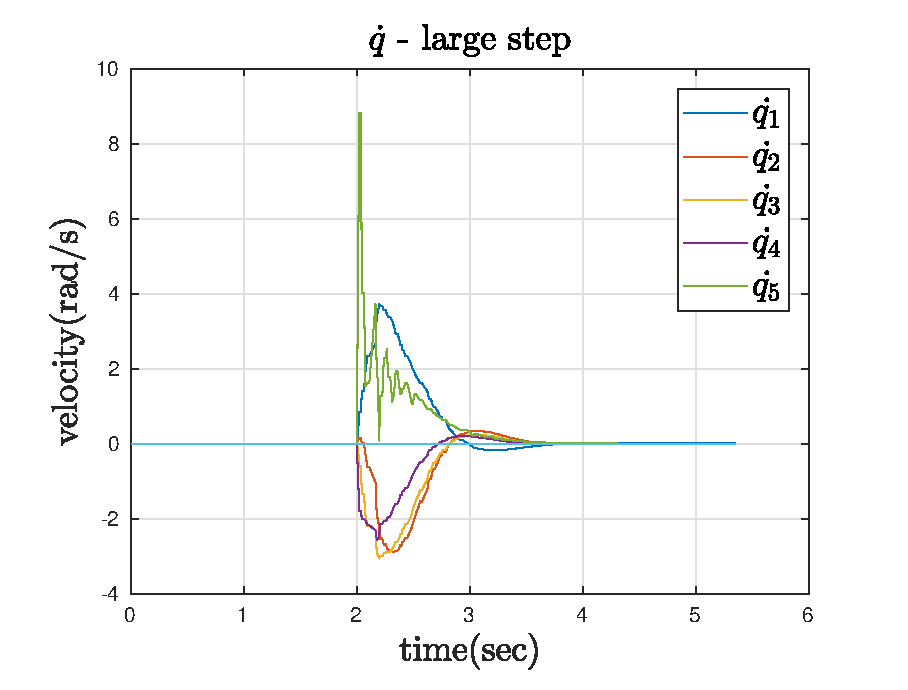
\includegraphics[width = 1.15\linewidth]{img/LSqdot.eps}
        \caption{ }
    \end{subfigure}
    ~ 
    \begin{subfigure}[htbp]{0.45\textwidth}
        \centering
        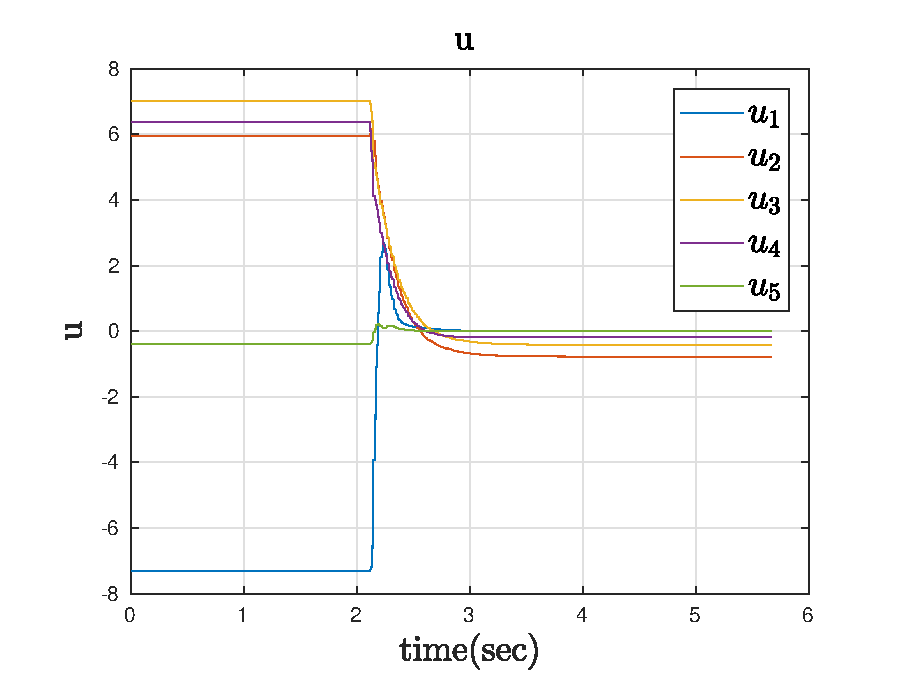
\includegraphics[width = 1.15\linewidth]{img/LSu.eps}
        \caption{ }
    \end{subfigure}
    ~
    \begin{subfigure}[htbp]{0.45\textwidth}
        \centering
        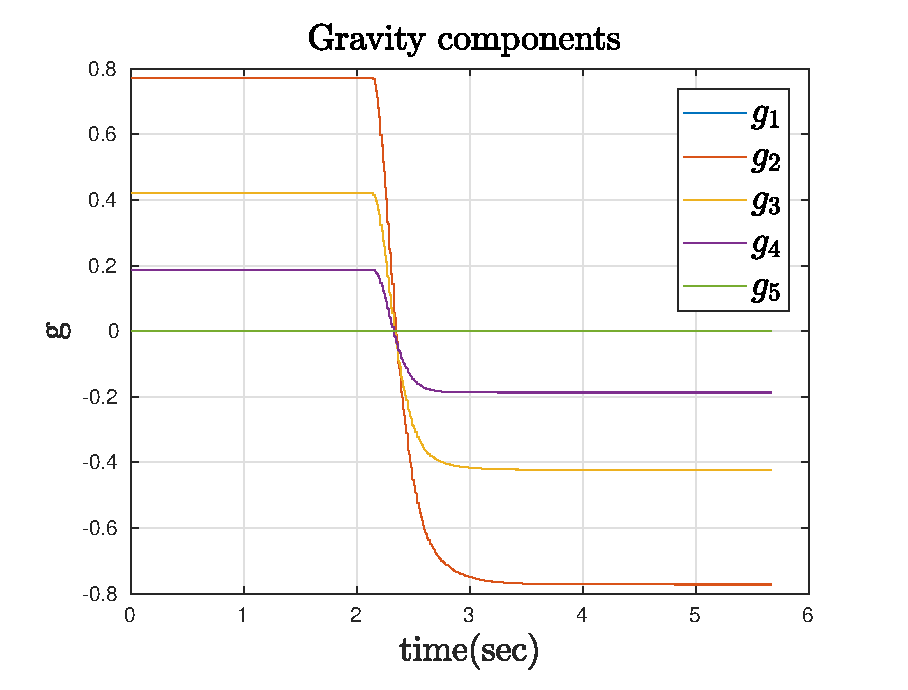
\includegraphics[width = 1.15\linewidth]{img/LSgrav.eps}
        \caption{ }
    \end{subfigure}
    \caption{Different plots of recorded data when a large step in desired joint angles is introduced}
    \label{fig:LS}
\end{figure*}

In \figref{fig:LS} different data is plotted from a random configuration to a some kind of inverse position such that every joint get to move. The step is rather large and because the intention of the robot arm is to do set point tracking some overshoot is therefore accepted for this case. By looking at the plots, the results looks good. One thing that could be better is the joint velocity of last joint which seems a bit unstable. Additional tuning to try to avoid the ugly input and joint velocity of the fifth joint results in slow convergence of the joint angle. Since the moments of inertia is very low and Gazebo handles low inertia very bad, so this effect is assumed to be because of this and the when implementing this on the real robot it is expected that this effect will not be a problem. From \figref{fig:LSq} one can see $q_5$ converges rather smooth and the gains will be used for further testing. It may be worth to mention that when doing set point tracking the steps are not that large and the gains can be altered for better performance.  





